\subsubsection{Mockups}
Für die Erstellung der Mockups hat das Projektteam das Tool Figma verwendet. Innerhalb eines geteilten Workspace wurden erste Entwürfe für die fünf verschiedenen Menüs der Applikation erstellt. Damit wird gezeigt, welche Funktionen eine solche App haben soll und wie das Design aussehen könnte.\\

\paragraph{Map}Der Tab „Map“ dient zur Darstellung der verfügbaren Möglichkeiten zur Lagerung von Fahrrädern in der Umgebung auf einer Karte. Mit einem Marker wird ein Fahrradturm dargestellt. Außerdem soll die Verfügbarkeit von freien Plätzen dargestellt werden.\\

\begin{figure}[ht]
  \centering
  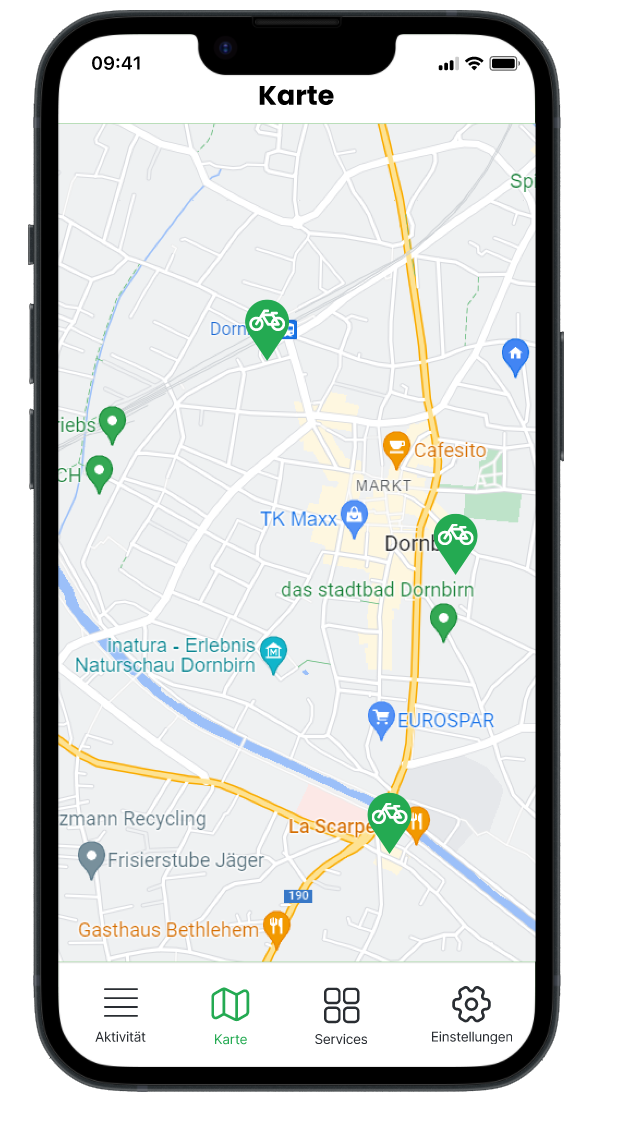
\includegraphics[width=0.3\textwidth]{images/app_mock_map}
  \caption{Mockup vom Screen Map}
  \label{fig:screenmap}
\end{figure}

\paragraph{Tower}Der Tab „Fahrradturm“ dient zur Anzeige folgender Informationen:
•	Karte mit Standort des Turmes
•	Anzahl verfügbaren Lagerungsmöglichkeiten
•	Bereits vom User bei diesem Turm gelagerte Gegenstände 
•	Möglichkeit zum Einlagern von einem weiteren Rad oder Gegenstand
 \\

\begin{figure}[ht]
  \centering
  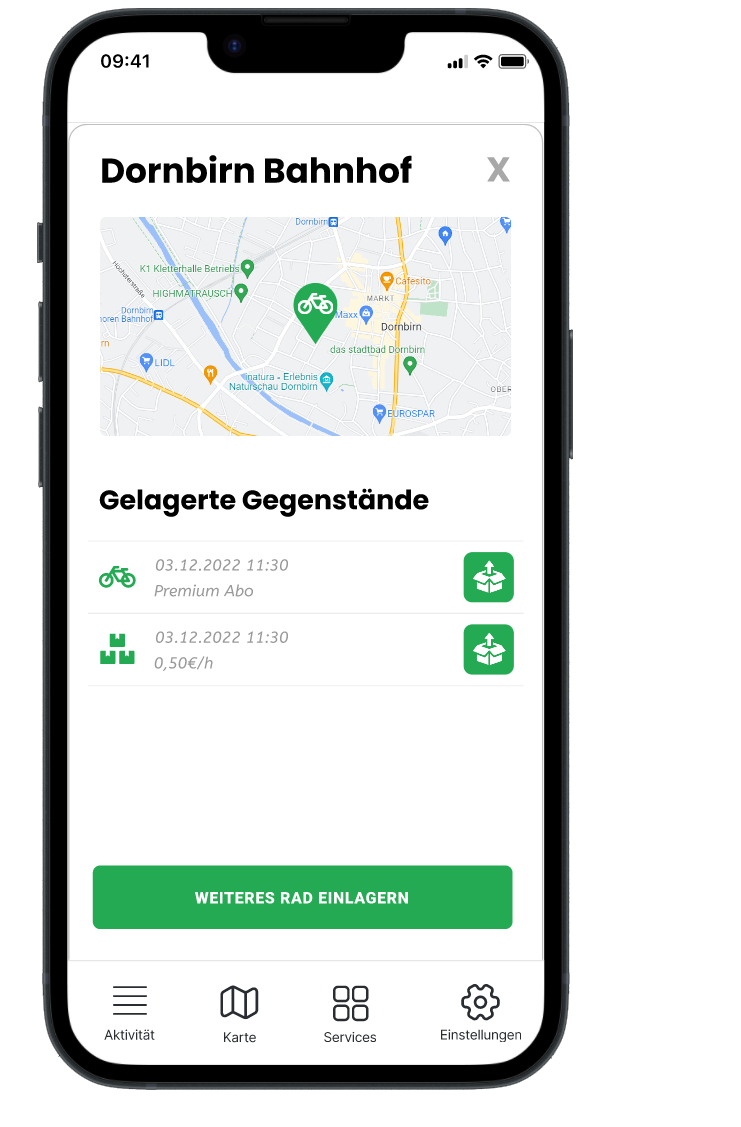
\includegraphics[width=0.3\textwidth]{images/app_mock_tower}
  \caption{Mockup vom Screen Tower}
  \label{fig:screentower}
\end{figure}

\begin{figure}[h]
  \centering
  
  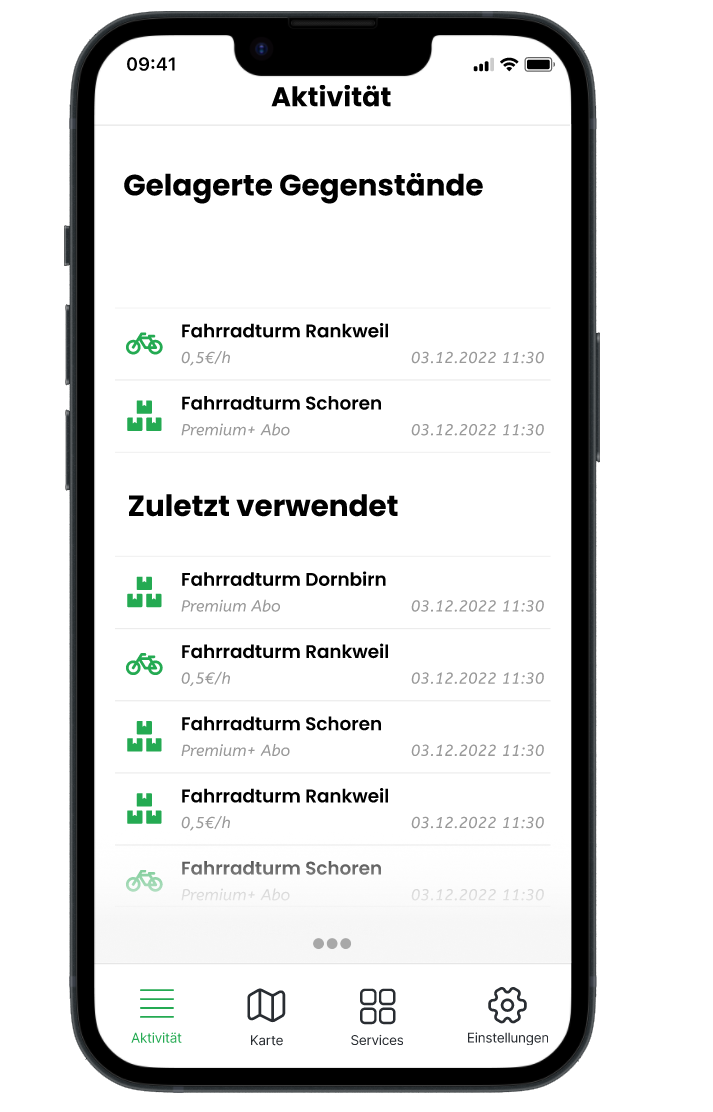
\includegraphics[width=0.15\textwidth]{images/app_mock_objects}
  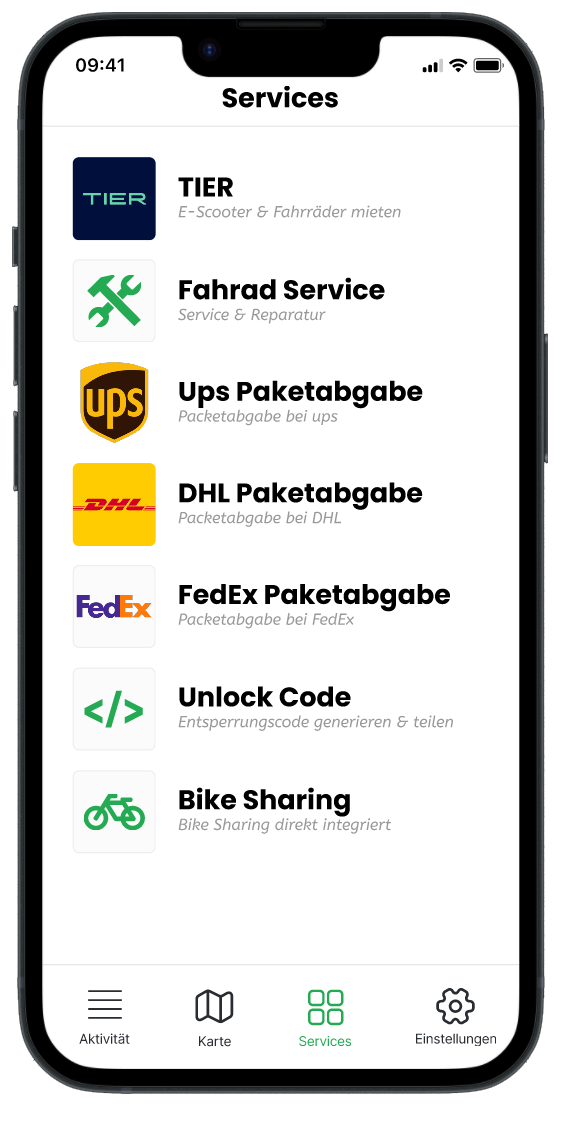
\includegraphics[width=0.15\textwidth]{images/app_mock_services}
  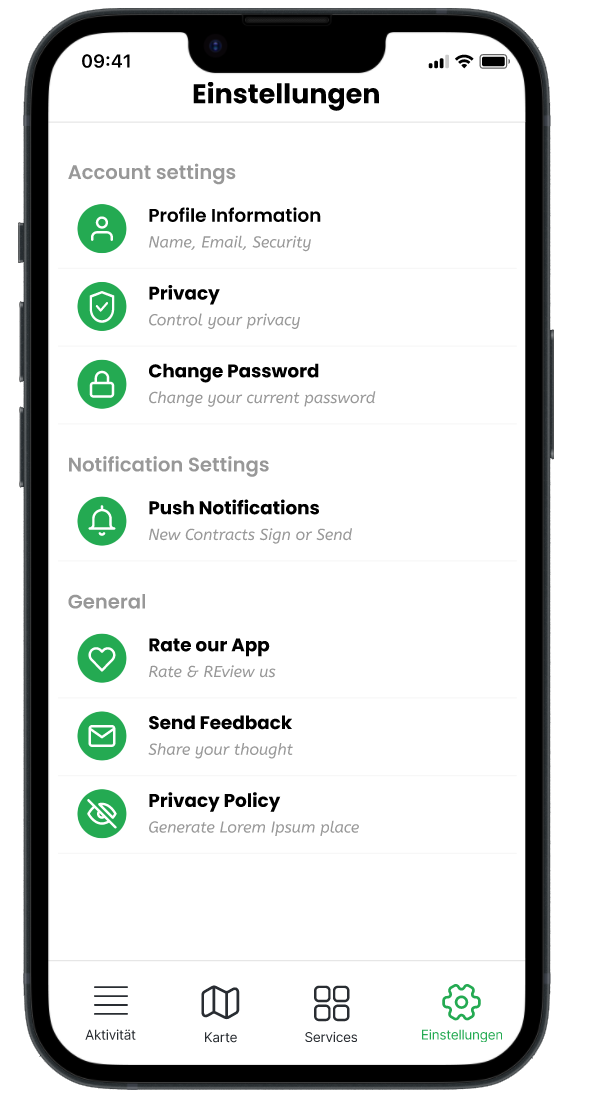
\includegraphics[width=0.15\textwidth]{images/app_mock_settings}
  \caption{App Mockup}
  \label{fig:app_mockup}
\end{figure}